\documentclass{article}
\usepackage{pgfplots}
\usepackage{../packages/intervalles}
\usepackage{tikz}
\pgfplotsset{compat=1.18}
\usepackage{tkz-tab}
\usetikzlibrary{babel,arrows,calc,fit,patterns,plotmarks,shapes.geometric,shapes.misc,shapes.symbols,shapes.arrows,shapes.callouts, shapes.multipart, shapes.gates.logic.US,shapes.gates.logic.IEC, er, automata,backgrounds,chains,topaths,trees,petri,mindmap,matrix, calendar, folding,fadings,through,positioning,scopes,decorations.fractals,decorations.shapes,decorations.text,decorations.pathmorphing,decorations.pathreplacing,decorations.footprints,decorations.markings,shadows}
\begin{document}

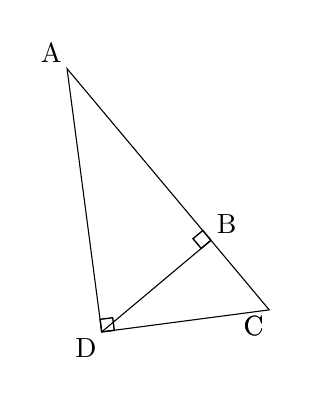
\begin{tikzpicture}[baseline,scale = 0.4]

    \tikzset{
      point/.style={
        thick,
        draw,
        cross out,
        inner sep=0pt,
        minimum width=5pt,
        minimum height=5pt,
      },
    }
    \clip (-4.46,-5.83) rectangle (3.71,5.13);
    	\draw[color={black}] (-3.21,3.83)--(3.21,-3.83)--(-2.11,-4.53)--cycle;
	\draw[color ={black}] (-2.11,-4.53)--(1.36,-1.62);
	\draw[color={black},line width = 0.5] (1.36,-1.62)--(1.1,-1.31)--(0.79,-1.57)--(1.05,-1.88)--cycle;
	\draw[color={black},line width = 0.5] (-2.11,-4.53)--(-2.16,-4.13)--(-1.76,-4.08)--(-1.71,-4.48)--cycle;
	\draw [color={black}] (-3.71,4.33) node[anchor = center,scale=1, rotate = 0] {A};
	\draw [color={black}] (1.86,-1.12) node[anchor = center,scale=1, rotate = 0] {B};
	\draw [color={black}] (2.71,-4.33) node[anchor = center,scale=1, rotate = 0] {C};
	\draw [color={black}] (2.71,-4.33) node[anchor = center,scale=1, rotate = 0] {C};
	\draw [color={black}] (-2.61,-5.03) node[anchor = center,scale=1, rotate = 0] {D};

\end{tikzpicture}

\end{document}

